\documentclass[a4paper,12pt]{ctexart}
%Coded UTF-8, To compile, use xelatex->biber->xelatex->xelatex
\usepackage{amsmath, amsfonts, amssymb}
\usepackage{mathrsfs}
\usepackage[url = false, doi = false, backend=biber,style=gb7714-2015,gbalign=gb7714-2015,gbpub=false,gbmedium=false]{biblatex} 
\addbibresource{ref.bib}
\addbibresource{ref2.bib}
\usepackage{indentfirst}
\usepackage{graphicx}
\usepackage{subfigure}
\usepackage{titling}  
\usepackage{multicol}
\usepackage{booktabs} 
\usepackage{xcolor}
\usepackage{hyperref}
\hypersetup{linkbordercolor=blue,anchorcolor=blue,citecolor=green}
\usepackage{multirow} 
\usepackage{stfloats}
\usepackage{enumerate}
\usepackage[top=1.25in, bottom=1.25in, left=1.5in, right=1.5in]{geometry}
\title{建立非禁闭势场中非平衡态统计的尝试}
\author{蔡智明,江浩楠,李昊天,陆雨航,王乾朔,周子正}
\date{\today}


\begin{document}
    \maketitle
    \noindent\rule{\textwidth}{0.5pt}

    {\heiti \noindent \textbf{摘要}\ \ } 
    {\kaishu 一般讨论的宏观系统相当于放置在具有有限体积的紧闭无限深势阱内部。本文讨论了非禁闭势场中存在的问题,尝试讨论了这种情况下的弛豫过程,在一维布朗运动背景下讨论了涨落定理、涨落耗散定理,通过数值方法对结果进行了一定程度的检验,并讨论了研究的局限性。}

    {\heiti \noindent \textbf{关键词}\ \ } {\kaishu \small 非禁闭势能,非平衡统计,一维布朗运动,涨落定理,涨落耗散定理}

    \noindent\rule{\textwidth}{0.5pt}

    %蔡写一下平衡部分,把题目背景也写一下
    %江王写一下Brownian部分,引入布朗运动方程,参考Aghion..重点讲pdf为啥是这个形式
    %周写一下涨落耗散定理
    %李写一下具体计算,把涨落定理形式给出来。对一般形式引用Strei..后面的结果。蔡简单解释一下附加项
    %周陆共同完成一下模拟计算,主要是分布结果,涨落定理..
    %周/陆写一下结论
    %蔡你找个人和你一起写一下讨论,主要包括涨落耗散定理高阶V导数。利用了布朗运动的局限性。并且简单讨论一下相互作用是1/r的问题。


    %各部分同学去掉自己部分注释尝试编译
 
    \section{题目分析与基本假设}
题目内容如下:
\textit{
    宏观系统从任意初态通过驰豫过程演化到内秉平衡态是有条件的,所需的条件是系统必须被束缚在有限的容器内。从物理上看,这相当于要求将宏观系统放置在具有有限体积的紧闭无限深势阱内部。若将系统放置在一个并非完全禁闭的势阱内,例如置于引力场中(势函数在无限远处趋于平坦,非禁闭),试研究相应的驰豫过程所对应的非平衡演化。对这样的系统是否可以建立相应的涨落定理以及涨落耗散定理?
    }

首先,在  D  维空间中,我们考虑一个在无穷远处趋于0且各向同性的单势阱,故在球坐标下势能  $V(r)$  随径向坐标$r$  变化图像大致如下图所示:
\begin{figure}[htbp]
  \centering
  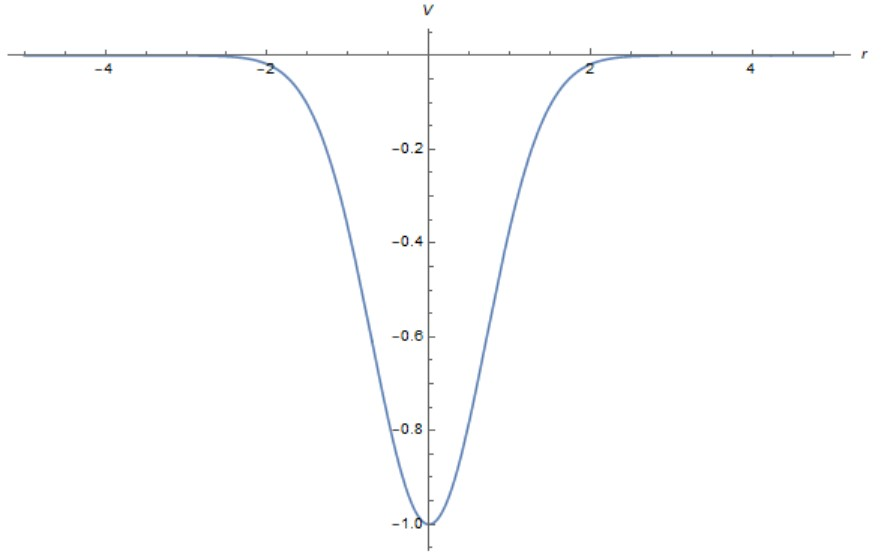
\includegraphics[width=0.8\linewidth]{figs/potential.jpg}
  \caption{势能  $V(r)$  的示意图}
\end{figure}

当  $V(r)$  为有限深方势阱时,我们可以自然地定义势阱的边界。当  $V(r)$  是光滑函数,我们可以人为地取某个函数固定的势能值  $V_{0}$,并认为当粒子势能小于  $V_{0}$  时,粒子处于势阱内。这样,势阱内的粒子构成一个开放系。

为了方便解决问题,我们引入如下两个假设:

\textbf{1.假设存在一个足够大的孤立系,使得系统总粒子数和能量守恒。}

我们在处理开放系时,都是将开放系置于一个外界大热库中,并认为开放系与大热库一起组成一个孤立系。当粒子可以达到无穷远处时,这样的处理并不显然。但考虑到我们可以观测的时空范围是有限的,上述假设总是合理的。而且,因为我们测量能量时的分辨率是有限的,所以我们总可以找到一个足够大的空间,使得内部的能量也是守恒的。

\textbf{2.假设孤立总系存在一个内禀平衡态,且系统会自发向内禀平衡态演化。}

对于一个粒子可以达到无穷远的系统,平衡态未必存在,这依赖于势能衰减的速度,在势能衰减不够快的情况下,粒子可能都驰豫到无穷远处。在我们的讨论中,假设系统存在平衡态。并且,根据后文数值模拟的结果,在长时间近似下,势场中的粒子分布基本不发生改变,故上述假设是合理的。

此外,为了简单起见,我们只考虑经典系统,满足玻尔兹曼近似$N\rightarrow\infty$。 
    \section{内禀平衡态的性质}
我们将势阱内的开放系作为我们讨论的对象。

由于我们讨论的是经典气体系统,故在平衡态时,气体满足玻尔兹曼分布,即
\begin{equation}\label{3.62}
  \mathrm{d} N(\boldsymbol{q}, \boldsymbol{p}) \approx \frac{1}{h^{D}} \mathrm{e}^{[\mu-\epsilon(\boldsymbol{q}, \boldsymbol{p})] / k_{0} T} \mathrm{~d} \mu(\boldsymbol{q}, \boldsymbol{p})
\end{equation}
其中,$\mathrm{d} N(\boldsymbol{q}, \boldsymbol{p})$  表示相空间  $(\boldsymbol{q}, \boldsymbol{p})$  附近的粒子数。$\mu-\epsilon(\boldsymbol{q}, \boldsymbol{p})$  是粒子在相空间  $(\boldsymbol{q}, \boldsymbol{p})$ 处的的能量,在非相对论情况下,  $\epsilon(\boldsymbol{q}, \boldsymbol{p})=\frac{\langle\vec{p}, \vec{p}\rangle}{2 m}+V(q)$。

将能量的表达式代入玻尔兹曼分布中并积分,得到粒子数分布。由于我们考虑的系统是势阱内的粒子,故积分区域为 $-\sqrt{2(V_{0}-V(q))}<p<\sqrt{2(V_{0}-V(q))},-q_{0}<q<q_{0}$,$q_{0}$  满足  $V(q_{0})=V_{0}$.
$$
N=\int_{-q_{0}}^{q_{0}} e^{-\frac{V(q)}{k_{0}T}}A_{D-1}q^{2} d q \frac{e^{\mu}}{h^{D}} \cdot \int_{-\sqrt{2\left(V_{0}-V(q)\right)}}^{\sqrt{2\left(V_{0}-V(q)\right)}} e^{-\frac{p^{2}}{2 m k_{0} T}} p^{2} A_{ D-1} dp
$$
代入特定的势能表达式,即可得到平衡态时势阱内粒子数与温度的关系。
\section{非禁闭势中的玻尔兹曼方程}
为了得到非禁闭势中的演化情况,让我们考虑非禁闭势情况下的玻尔兹曼方程。由于我们考虑的空间区域是开放的,在写出玻尔兹曼方程时,要再附加上因粒子进出导致的微观态分布函数变化项:
\begin{equation}
\frac{\partial f}{\partial t}=\left(\frac{\partial f}{\partial t}\right)_{\text {扩散 }}+\left(\frac{\partial f}{\partial t}\right)_{\text {漂移 }}+\left(\frac{\partial f}{\partial t}\right)_{\text {散射 }}+\left(\frac{\partial f}{\partial t}\right)_{\text {进出 }}
\end{equation}
我们考虑  $\left(\frac{\partial f}{\partial t}\right)_{\text {进出 }}$  的行为。由于我们考虑的是无穷小时间间隔内粒子的进出,故只有边界上的粒子对  $\left(\frac{\partial f}{\partial t}\right)_{\text {进出 }}$  有贡献。在势阱内部,系统仍满足平移对称性,故势阱内部玻尔兹曼方程不变。而对于势阱的边界,  $\left(\frac{\partial f}{\partial t}\right)_{\text {进出 }}$  会造成系统边界条件的改变。

在长时间条件下,总的粒子数改变量相当于,
\begin{equation}
  \left( \Delta f \right) _{\text{总}}\left( t \right) =\int_0^t{d\tau \oint_{V\left( \vec{q} \right) <V_0}{d\vec{q}\int_{\mathrm{k}_{0}\left( \vec{q} \right)}^{+\infty}{dk\ \mathcal{A}_nk^{n-1}f\left( \vec{q},k,\tau \right)}}}
\end{equation}
其中$\mathrm{k}_{0}(\vec{q}) = \sqrt{2m(V_0-V(\vec{q}))/\hbar^2}$,$\mathcal{A}_n$是n维空间中n-1维单位球面积。



    \section{一维布朗运动}
%TODO

\section{一维布朗运动的分布函数}
我们接下来尝试讨论一维布朗运动的分布函数,令
$\mathcal{O}[x(t)]=I\left(x_{1}<x(t)<x_{2}\right)$表示单个粒子在$\left(x_{1}, x_{2}\right)$之间存在的时间,如果满足括号内的条件则$I(\cdots)=1$,不满足则为0.
因此可以沿着粒子的轨迹$x(t)$,通过$I(\cdots)$在值0到1之间的变换,相应的得到粒子是否在区域$\left(x_{1}, x_{2}\right)$中。而这个可观测值I的集合平均,
可以表示为:
\begin{equation}
\left\langle I\left(x_{1}<x(t)<x_{2}\right)\right\rangle=\int_{0}^{\infty} I\left(x_{1}<x<x_{2}\right) P_{t}(x) \mathrm{d} x \sim \int_{x_{1}}^{x_{2}} e^{-\beta V(x)} / \mathcal{Z}_{t}\mathrm{d}x
\end{equation}
当系统处于热平衡时,该式即变为粒子出现在区间$\left(x_{1}, x_{2}\right)$ 的概率,粒子在该区域内停留的时间记为滞留时间:$t_{x_{1}<x<x_{2}}$
经过一段长时间的观测,由Boltzmann测度可得:
\begin{equation}
\lim _{t \rightarrow \infty}\frac{t_{x_{1}<x<x_{2}}}{ t}=\frac{\int_{x_{1}}^{x_{2}} e^{-\beta V(x)} \mathrm{d} x}{Z}
\end{equation}
由Boltzmann-Gibbs理论的Birkhoff遍历假设可知,观测得到有限时间平均值为:
\begin{equation}
\frac{t_{x_{1}<x<x_{2}}}{t}=\frac{\int_{0}^{t} I\left(x_{1}<x(t)<x_{2}\right) \mathrm{d} t}{t}
\end{equation}
该式通过对一组路径求平均获得,而每个对应的轨迹都有自己的滞留时间。因此有:\begin{equation}
\left\langle\frac{t_{x_{1}<x<x_{2}}}{t}\right\rangle=\frac{\left\langle\int_{0}^{t} I\left(x_{1}<x(t)<x_{2}\right) \mathrm{d} t\right\rangle}{t}
\end{equation}
在该值的计算中,可以利用公式:
\begin{equation}
\left\langle I\left(x_{1}<x(t)<x_{2}\right)\right\rangle=\int_{x_{1}}^{x_{2}} P_{t}(x) \mathrm{d} x
\end{equation}
在条件:$\mathcal{Z}_{t}=$ $\sqrt{\pi D t}$下可以得到:
\begin{equation}
\left\langle\frac{t_{x_{1}<x<x_{2}}}{t}\right\rangle \sim \frac{1}{t} \int_{0}^{t} \mathrm{~d} t \frac{\int_{x_{1}}^{x_{2}} e^{-\beta V(x)} \mathrm{d} x}{\mathcal{Z}_{t}}=
2 \frac{\int_{x_{1}}^{x_{2}} \exp [-\beta V(x)] \mathrm{d} x}{\mathcal{Z}_{t}}
\end{equation}
2倍的因子是时间积分的结果,由于长时间的限制,下标可以写作0。
现在考虑的情况为一维情况,当x趋于远处,势趋于平坦的势阱。可以界定一个范围$l_{1}$,当$x>l_{1}$时,
将该区域的势能视为0,即代表在$0<x<l_{1}$处,并且有$\exp \left(-x^{2} / 4 D t\right) \sim 1$。
由粒子的扩散性质,在$0\sim l_{1}$处。粒子由势阱中逃逸,向束缚力趋于零的区域扩散。(需要更改)
但是在$x>l_{1}$区域的粒子同时也会向着内部区域扩散,从而重新返回到非零势能区域内。
这说明任何粒子,无论粒子到达了哪个区域当中,都会回归到$x<(l_{1})$区域内。那么以$N\gg1$的粒子实验,经过有限时间后总可以在$(x>l_{1})$以外的区域发现它,也总可以观察到粒子的返回,所以在边界$(x=l_{1})$附近总有一部分不可忽略的粒子存在。
(与本文所讨论的模型相符:经过有限长的时间,由于边界是时间的二分之一次方形式,边界总可以到达足够的长度使得所有粒子回归的概率为1。)(可以更改)
现在考虑一个可观察的时间$\mathcal{O}[x(t)]$,
对于玻尔兹曼因子它是可积分的,那么有:\begin{equation}
\langle\mathcal{O}(x)\rangle=\frac{\int_{0}^{\infty} \mathcal{O}(x) \exp [-\beta V(x)] \mathrm{d} x}{\mathcal{Z}_{t}}
\end{equation}
时间总体平均值为:
\begin{equation}
\langle\overline{\mathcal{O}[x(t)]}\rangle=2\langle\mathcal{O}(x)\rangle
\end{equation}
2倍的因子实际为扩散性质的结果,它直接导致对时间相关配方函数的积分。这其实是伯克霍夫定律的推广(细说一下伯克霍夫定律)。
而这个时间总体平均值等于长时间限制中的整体平均。

之前提到过,时间平均值随着粒子的轨迹变化,讨论在不同轨迹间的波动。
考虑方程
\begin{equation}
\mathcal{O}[x(t)]=I\left(x_{1}<x(t)<x_{2}\right)
\end{equation}
出于简单,令$x_{1}=0$,则$\left(x_{1}, x_{2}\right)$变为了$\left(0, x_{2}\right)$。定义滞留时间$\tau^{\mathrm{in}}$记为\begin{equation}
I\left(x_{1}<x(t)<x_{2}\right)=1
\end{equation}
离散时间$\tau^{\mathrm{out}}$当$I\left(x_{1}<x(t)<x_{2}\right)=0$。
因此在
$\left(0, x_{2}\right)$
区域内粒子处于两种状态的序列为:
\begin{equation}
\left\{\tau_{1}^{\mathrm{in}}, \tau_{1}^{\mathrm{out}}, \tau_{2}^{\mathrm{in}}, \tau_{2}^{\mathrm{out}}, \cdots\right\}
\end{equation}
由于朗之万方程的时间相关性随时间的增长成指数倍形式下降,因此这些时间可被视为互相独立,相同分布的随机变量。
使用$\psi_{\text {out } / \text { in }}(\tau)$来作为$\tau^{\mathrm{out}} 和\tau^{\mathrm{in}}$概率密度函数,在平坦势的情形下$\tau^{\mathrm{out}} $的概率密度函数正比于$t^{-3/2}$($\tau^{out}\gg\tau^{in}$所以$\tau^{out}\sim t$)。
对于固定的测量时间t而言,假设粒子由内部区域到外部区域的次数总共有n 次,那么当t很大时,由于离散时间远大于滞留时间。
因此n的分布由离散时间来确定。
可以重新定义:$I\left(x_{1}<x(t)<x_{2}\right)$的时间平均值记为滞留时间的总和除以测量时间t:
\begin{equation}
\bar{I}=\sum_{i=1}^{n} \tau_{i}^{\mathrm{in}} / t
\end{equation}
注意有效逗留时间:
\begin{equation}
\left\langle\tau_{\mathrm{eff}}\right\rangle=\int_{0}^{t} \tau \psi_{\mathrm{out}}(\tau) \mathrm{d} \tau \propto t^{1 / 2}
\end{equation}
所以有:
\begin{equation}\langle n\rangle \sim t /\left\langle\tau_{\text {eff }}\right\rangle \propto t^{1 / 2}
\end{equation}
再反过来看
\begin{equation}
\langle\bar{I}\rangle \simeq\left\langle\tau^{\mathrm{in}}\right\rangle\langle n\rangle / t
\end{equation}
有时间平均值与$t^{-1/2}$成正比。
现在考虑测量时间t很长时的情况,对于任何j≠i,都有:
\begin{equation}
\left\langle\left(\tau_{i}^{\mathrm{in}}\right)^{2}\right\rangle=\left\langle\left(\tau_{j}^{\mathrm{in}}\right)^{2}\right\rangle
\end{equation}
以及
\begin{equation}
\left\langle\tau_{i}^{\mathrm{in}} \tau_{j}^{\mathrm{in}}\right\rangle=\left\langle\tau_{i}^{\mathrm{in}}\right\rangle^{2}
\end{equation}
可以得到:
\begin{equation}
\left\langle\bar{I}^{2}\right\rangle =\frac{\left\langle\left(\sum_{i=1}^{n} \tau_{i}^{\mathrm{in}}\right)^{2}\right\rangle}{t^{2}}
=\frac{\langle n\rangle\left\langle\left(\tau^{\mathrm{in}}\right)^{2}\right\rangle+\langle n(n-1)\rangle\left\langle\tau^{\mathrm{in}}\right\rangle^{2}}{t^{2}} .
\end{equation}
考虑时间平均值的方差:
\begin{equation}
\left\langle(\bar{I})^{2}\right\rangle-\langle\bar{I}\rangle^{2}=\frac{\left\langle\left(t_{r}\right)^{2}\right\rangle-\left\langle t_{r}\right\rangle^{2}}{t^{2}}=\frac{\left\langle n^{2}\right\rangle-\langle n\rangle^{2}}{t^{2}}\left\langle\tau^{\mathrm{in}}\right\rangle^{2}+\frac{\langle n\rangle}{t^{2}} \underbrace{\left[\left\langle\left(\tau^{\mathrm{in}}\right)^{2}\right\rangle-\left\langle\tau^{\mathrm{in}}\right\rangle^{2}\right]}_{\operatorname{Var}\left(\tau^{\mathrm{im}}\right)}
\end{equation}
由前文得到的n与t的关系,发现第二项相比于第一项可以忽略不计,再由
\begin{equation}
\langle\bar{I}\rangle \simeq\left\langle\tau^{\mathrm{in}}\right\rangle\langle n\rangle / t
\end{equation}
可以得到:
\begin{equation}
\frac{\left\langle\bar{I}^{2}\right\rangle-\langle\bar{I}\rangle^{2}}{\langle\bar{I}\rangle^{2}} \rightarrow \frac{\left\langle n^{2}\right\rangle-\langle n\rangle^{2}}{\langle n\rangle^{2}}
\end{equation}
将其继续到高阶矩,有:
\begin{equation}
\frac{\bar{I}}{\langle\bar{I}\rangle} \rightarrow \frac{n}{\langle n\rangle} \equiv \eta
\end{equation}
这表明在$\left(x_{1}, x_{2}\right)$区域内的滞留时间比上平均滞留时间,实际上等于在其平均值上粒子从滞留态到离散态的数目。可以得到$0<\eta $的概率密度函数\cite{godrecheStatisticsOccupationTime2001},结合$\psi_{\text {out }}(\tau) \propto \tau^{-3 / 2}$
可以得到:\begin{equation}
\operatorname{PDF}(\eta)=\frac{2}{\pi} e^{-\eta^{2} / \pi}
\end{equation}
虽然它有与高斯中心极限定理有关的形式,但是实际上PDF是关于Mittagle-Leffler分布,它与L有关。
Aaronson-Darlin-Kac定理预测在无穷测度的过程的时间平均分布将由Mittag-Leffler分布给出:
\begin{equation}
\mathscr{N}_{\alpha}(\eta)=\frac{\Gamma^{1 / \alpha}(1+\alpha)}{\alpha \eta^{1+1 / \alpha}} l_{\alpha, 0}\left[\frac{\Gamma^{1 / \alpha}(1+\alpha)}{\eta^{1 / \alpha}}\right], l_{\alpha, 0}(\#)
\end{equation}
为利维密度,指数α由$\psi_{\text {out }}(\tau) \propto \tau^{-1-\alpha}$ 给出,此时α=1/2,
那么在我们的物理模型下考虑n个独立的同分布随机变量,根据levy中心极限定理\cite{metzlerRandomWalkGuide2000},相应的概率密度函数Probability Density Function(PDF)为:\begin{equation}
l_{1 / 2,0}(\tau)=\frac{1}{2 \sqrt{\pi}} \tau^{-3 / 2} \exp \left(-\frac{1}{4 \tau}\right)
\end{equation}
现在引入随机变量$y=\sum_{i=1}^{n} \tau_{i} / n^{2}$,由于
\begin{equation}
t=\sum_{i=1}^{n} \tau_{i}
\end{equation}
因此$y=t / n^{2}$,
可以得到PDF关于y的函数形式为:
\begin{equation}
\operatorname{PDF}(n)=\operatorname{PDF}(y)\left|\frac{\mathrm{d} y}{\mathrm{~d} n}\right|=
l_{1 / 2,0}\left(\frac{t}{n^{2}}\right)\left|\frac{2 t}{n^{3}}\right|=\frac{1}{\sqrt{\pi t}} \exp \left(-\frac{n^{2}}{4 t}\right)
\end{equation}
    \section{一维布朗运动模型下\\非禁闭背景势场的涨落定理}
研究外加势场作用下的过阻尼布朗运动粒子,其郎之万方程可以写为
\begin{equation}
\dot{x}_{t}=-\frac{V^{\prime}\left(x_{t}, \lambda_{t}\right)}{\gamma}+\sqrt{2 D} \xi_{t}
\label{equ:langzw}
\end{equation}
其中$V(x_t,\lambda_t)$依赖于外部控制的参数$\lambda_t$,并且$V(x_t,\lambda_t)$是一个在无穷远处渐进平坦的势阱,其衰减的速度不慢于$1/x$,有
\begin{equation}
\lim\limits_{x\rightarrow\pm\infty}V(x_t,\lambda_t)=0
\end{equation}
$D$ 为扩散常数,$\gamma$ 为阻力,$\xi_t$ 为高斯白噪音,满足
\begin{equation}
\left\langle\xi_t\right\rangle=0
\end{equation}
\begin{equation}
\left\langle\xi_{t} \xi_{t^{\prime}}\right\rangle=\delta\left(t-t^{\prime}\right)
\end{equation}
系统的PDF$P(x,t)$满足的Fokker-Planck方程为
\begin{equation}
\frac{\partial}{\partial t}P(x,t)=-\frac{\partial}{\partial x}\frac{\langle\delta x\rangle}{\delta t}P(x,t)+\frac{\partial^2}{\partial t^2}\frac{1}{2}\frac{\langle(\delta x)^2\rangle}{\delta t}P(x,t)
\end{equation}
其中$\delta x$可以对式(\ref{equ:langzw})两边在$\delta t$时间内积分,得到
\begin{equation}
\delta x=-\frac{V'(x_t,\lambda_t)}{\gamma}\delta t+\sqrt{2D}\int^{t+\delta t}_{t}\xi_{t'}\mathrm{d}t'
\end{equation}
两边对系综取平均,利用白噪声均值为0的特点得到
\begin{equation}
\frac{\langle\delta x\rangle}{\delta t}=-\frac{V'(x_t,\lambda_t)}{\gamma}
\end{equation}
对于$\frac{\langle(\delta x)^2\rangle}{\delta t}$,首先将$\delta x$取平方,同时注意到$\delta t$项的贡献为0,因此只剩下最后一项有贡献,有
\begin{equation}
\frac{\langle(\delta x)^2\rangle}{\delta t}=\lim\limits_{\delta t\rightarrow0}\frac{2D}{\delta t}\int^{t+\delta t}_t\mathrm{d}t'\int^{t+\delta t}_t\mathrm{d}t''\left\langle\xi_t\xi_{t'}\right\rangle=2D
\end{equation}
代入Fokker-Planck方程得
\begin{equation}
\partial_{t} P(x, t)=L P(x, t)
\end{equation}
其中$L$是Fokker-Planck算符
\begin{equation}
L=\left(D \partial_{x}^{2}+\frac{1}{\gamma} \partial_{x} V^{\prime}\right)
\label{equ:FPoper}
\end{equation}
对于一个固定的$\lambda_t$和足够长的时间下,$P(x,t)$会收敛于
\begin{equation}
P_{\mathrm{GB}}\left(x, t, \lambda_{t}\right)=\frac{e^{-\frac{x^{2}}{4 D t}-\beta V\left(x, \lambda_{t}\right)}}{N\left(t, \lambda_{t}\right)}
\label{equ:PDF}
\end{equation}
其中$\beta=\frac{1}{\mathrm{k}_{0}T}$,$N(t,\lambda_t)$是归一化常数,满足
\begin{equation}
N\left(t, \lambda_{t}\right)=\int_{-\infty}^{\infty} e^{-\frac{x^{2}}{4 D t}-\beta V\left(x, \lambda_{t}\right)} \mathrm{d} x
\end{equation}
我们将(\ref{equ:PDF})与之前得到的式(\ref{PDFjiang})对比,我们发现两者都有一个高斯型的因子,只不过这里在e指数上多了一项与势场有关的因子。

考虑一个特殊情况:在$t=0$时,粒子全部被置于势阱内。从$t=0$到$t=t_0$这段时间内,系统处于弛豫使得在$t=t_0$时概率密度大致可以由$P_{\mathrm{GB}}(x,t_0)$给出。从$t=t_0$到$t=t_1$,势场由于外部控制的参数$\lambda_t$介入而发生改变,直到$t=t_1$时势场停止变化,系统的概率密度重新回到弛豫过程的分布,如式(\ref{equ:PDF})所示。然而这种弛豫过程不会对最终的结果产生影响,在这种情况下,定义由$\lambda_t$产生的广义力\cite{streissnigWorkFluctuationTheorem2021}
\begin{equation}
F_{\lambda_t}=-\frac{\partial V(x_t,\lambda_t)}{\partial\lambda_t}
\end{equation}
由外部参数$\lambda_t$ 沿着时间$t$ 依赖的轨道所做的功可以利用功率对时间的积分表示为
\begin{equation}
W_{t}=-\int_{t_{0}}^{t} \dot{\lambda}_{\tau}F_{\lambda_{\tau}}\mathrm{d} \tau=\int_{t_{0}}^{t} \dot{\lambda}_{\tau} \frac{\partial V\left(x_{\tau}, \lambda_{\tau}\right)}{\partial \lambda_{\tau}} \mathrm{d} \tau=\int_{t_{0}}^{t} \frac{\partial V\left(x_{\tau}, \tau\right)}{\partial \tau} \mathrm{d} \tau
\label{equ:Wt}
\end{equation}

为了简单起见,我们考虑势的变化在瞬间完成,数学上可以表示为$V\left(x, \Theta\left(t-t_{0}\right)\right)$,这里可以很自然地把外部控制的参数$\lambda_t$表示为
\begin{equation}
\lambda_{t}=\Theta\left(t-t_{0}\right)
\end{equation}
定义
\begin{equation}
\Delta V(x):=V(x, 1)-V(x, 0)
\end{equation}
利用这一符号可以把势写为
\begin{equation}
V\left(x, \lambda_{t}\right)=V(x, 0)+\lambda_{t} \Delta V(x)
\label{equ:V-x-lambda}
\end{equation}
把式(\ref{equ:V-x-lambda})代入到式(\ref{equ:Wt})中,由于$\dot{\lambda}_t=\delta{t-t_0}$为一$\delta$函数形式,可以把依赖于轨迹的功$W_t$表示为变化前后在$x_{t_0}$处的势之差表示,得
\begin{equation}
W_{t}=\Delta V\left(x_{t_{0}}\right)
\end{equation}
利用$t=t_0$时的概率密度分布可以计算
\begin{equation}
\left\langle e^{-\beta W_{t}}\right\rangle=\int_{-\infty}^{\infty} e^{-\Delta \beta V(x)} P_{\mathrm{GB}}\left(x, t_{0}, 0\right) \mathrm{d} x=\frac{\int_{-\infty}^{\infty} e^{-\frac{x^{2}}{4 D t_{0}}-\beta V(x, 1)} \mathrm{d} x}{N\left(t_{0}, 0\right)}
\end{equation}
其中
\begin{equation}
N(t_0,0)=\int_{-\infty}^{\infty} e^{-\frac{x^{2}}{4 D t_{0}}-\beta V(x, 0)} \mathrm{d} x
\end{equation}
定义
\begin{equation}
\Delta G=-\beta \ln \left(\frac{N\left(t_{0}, 0\right)}{N\left(t_{0}, 1\right)}\right)=-\beta \ln \left(\frac{\int_{-\infty}^{\infty} e^{-\frac{x^{2}}{4 D t_{0}}-\beta V(x, 1)} \mathrm{d} x}{\int_{-\infty}^{\infty} e^{-\frac{x^{2}}{4 D t_{0}}-\beta V(x, 0)} \mathrm{d} x}\right)
\end{equation}
可以得到
\begin{equation}
\left\langle e^{-\beta W_{t}}\right\rangle=e^{-\beta \Delta G}
\end{equation}
与Jarzinski等式类似,这个结果不依赖于系统是否存在平衡态,更加一般的形式为
\begin{equation}
\langle W_{t}\rangle\geqslant\Delta G
\end{equation}
    \section{模拟分析}
根据式(\ref{equ:langzw}),单个布朗粒子在外势场下所满足的运动方程为:
$$
\dot{x}=-\frac{V^\prime\left( x_t,\lambda _t \right)}{\gamma}+\sqrt{2D}\xi _t
$$
其中,$\xi_t$为随机外力,如果仅在随机力作用下粒子随时间的变化将为高斯型分布,即为扩散的结果,也说明随机外力产生的是扩散运动;外势场的梯度对应着粒子的漂移运动,这个势场作为非禁闭势,将对粒子产生一定约束作用,形成一个存在的稳态分布$\gamma$代表摩擦对外力产生的减弱效应。

此处的运动方程形式上是常微分方程,但由于随机力存在,方程为一随机微分方程,需要考虑使用多粒子同时进行随机微分方程求解,其中随机力在对多粒子的平均中为0。同时考虑n个粒子,利用Euler–Maruyama方法\cite{vomscheidtKloedenPEPlaten1994},将随机微分方程在一定的时间区间上求解,我们可以得到每个粒子的运动过程,同时也能得到经过一定时间后,粒子在空间上的分布情况,如图(\ref{fig:sim-coordinate})所示。

\begin{figure}[H]
    \centering
    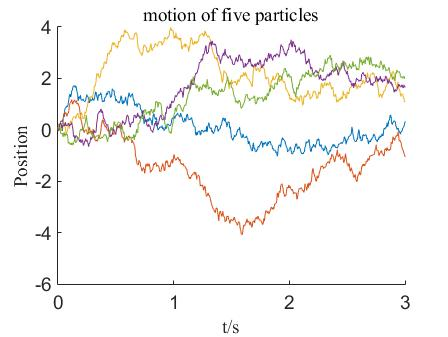
\includegraphics[width=0.8\linewidth]{figs/粒子坐标.jpg}
    \caption{前5个粒子的运动轨迹,模拟过程中选择$D=\gamma=\mathrm{k}_{0}T=1$,在$t_0=0.1 \text{s}$加入势场影响,时间间隔为0.005 s,粒子数$n=10000$。}
    \label{fig:sim-coordinate}
\end{figure}

在模拟中,我们选择势场$V$的形式为具有偏移的高斯型势场:
\begin{equation}
    V\left( x,\tau \right) =-A\left( \tau \right) e^{-\frac{\left( x-B\left( \tau \right) \right) ^2}{2}}
\end{equation}
为了验证之前所叙述的随机力对应扩散运动,同时还能在之后加入势场所产生的影响,我们选择$A(\tau)=\theta(\tau-t_0)$,其中$\theta$对应一个阶跃函数,表示在时间$t_0$之前没有势场影响,在$t_0$之后加入了势场的影响。为了能具体显示势场对漂移的影响,我们选择$B(\tau)=1$,可以直接展示势场对粒子运动的束缚作用。

\begin{figure}[H]
    \centering
    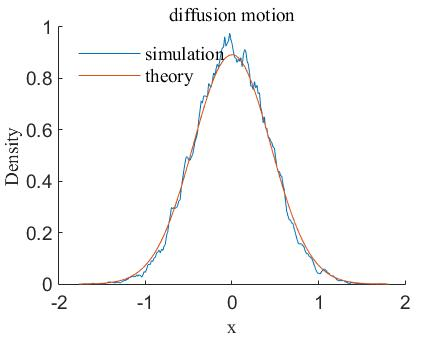
\includegraphics[width=0.8\linewidth]{figs/扩散运动.jpg}
    \caption{未加势场时,粒子的扩散运动}
    \label{fig:sim-no-V}
\end{figure}

如图我们可以看到不加势场时,粒子运动为一扩散运动,形成高斯型分布,满足:
\begin{equation}
    \varrho \left( x,t \right) =\frac{1}{\left( 4\pi Dt \right) ^{1/2}}\exp \left[ -\frac{\left( x-x_0 \right) ^2}{4Dt} \right]
\end{equation}

需要注意其中势场有一个单位偏移,在此处才能看到分布的偏移情况。能在图 (\ref{fig:sim-V})中观察到中心位置处于1的位置上,势场对粒子的约束作用满足我们之前推导得到的理论分布(\ref{equ:PDF})。

\begin{figure}[H]
    \centering
    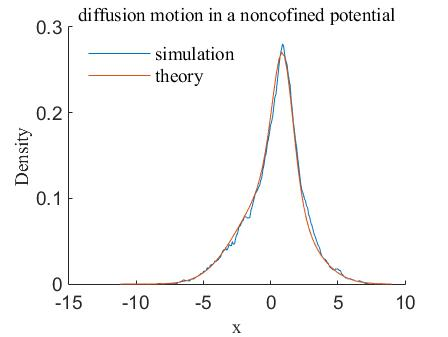
\includegraphics[width=0.8\linewidth]{figs/势场中的分布.jpg}
    \caption{加入势场后粒子的分布}
    \label{fig:sim-V}
\end{figure}
    \section{对非禁闭势场中涨落定理的讨论}
接下来,我们讨论非禁闭势场中涨落定理的更普遍情况。在文献\cite{streissnigWorkFluctuationTheorem2021}
中,给出了非禁闭势场中的涨落定理:
\begin{equation}\label{36}
\left\langle e^{-\beta\left[W_{t}-\int_{t_{0}}^{t}\left(\frac{k_{\mathrm{B}} T}{2 \tau}+\frac{x_{\tau} F\left(x_{\tau}, \lambda_{\tau}\right)}{2 \tau}\right) \mathrm{d} \tau-\Delta G\right]}\right\rangle=1
\end{equation}
利用数学上的詹森不等式,我们还可以得到如下结论:
\begin{equation}\label{37}
\left\langle W_{t}\right\rangle \geqslant \Delta G+\left\langle\int_{t_{0}}^{t}\left(\frac{k_{0} T}{2 \tau}+\frac{x_{\tau} F\left(x_{\tau}, \lambda_{\tau}\right)}{2 \tau}\right) \mathrm{d} \tau\right\rangle
\end{equation}
这个不等式给出了外界对系统做功统计平均值的一个下限。

首先,让我们比较非禁闭势场中涨落定理  $(\ref{36})$  与禁闭势场中的贾金斯基等式:
\begin{equation}\label{jia}
\left\langle e^{-\beta(W-\Delta F)}\right\rangle=1
\end{equation}

我们可以发现,这两个等式在形式上有相似之处,但有两点不同。首先,$(\ref{36})$  比  $(\ref{jia})$  多了一个依赖于轨道的积分项:
\begin{equation}
\int_{t_{0}}^{t}\left(\frac{k_{0} T}{2 \tau}+\frac{x_{\tau} F\left(x_{\tau}, \lambda_{\tau}\right)}{2 \tau}\right) \mathrm{d} \tau
\end{equation}
其次,$(\ref{36})$  中的  $\Delta G$  取代了  $(\ref{jia})$  中的  $\Delta F$,并且因为  $\Delta G$  中的  $N\left(t, \lambda_{t}\right)$  显含时间,  $\Delta G$  也会显含时间。这些不同点的根源都在于我们最初使用的概率密度分布函数  $P_{GB}$。

下面,我们计算在  $P_{GB}$  分布下  $\Omega_{t}$  的平均值。根据  $\Omega_{t}$  的定义式与  $P_{GB}$  分布下的平均值计算公式,并将  $P_{GB}$  的表达式代入,我们得到:
\begin{equation}
\begin{aligned}
&\left\langle\Omega_{t}\right\rangle_{\mathrm{GB}}=\int_{t_{0}}^{t} \mathrm{~d} \tau\left\langle f\left(x, \tau, \lambda_{\tau}\right)\right\rangle_{\mathrm{GB}} \\
&=\int_{t_{0}}^{t} \mathrm{~d} \tau \int_{-\infty}^{\infty} \mathrm{d} x f\left(x, \tau, \lambda_{\tau}\right) \frac{e^{-\frac{x^{2}}{4 D \tau}-\beta V\left(x, \lambda_{\tau}\right)}}{N\left(\tau, \lambda_{\tau}\right)}
\end{aligned}
\end{equation}
将朗之万方程代入得
$$
\left\langle\Omega_{t}\right\rangle_{\mathrm{GB}}=-\int_{t_{0}}^{t} \mathrm{~d} \tau \frac{1}{N\left(\tau, \lambda_{\tau}\right)} \int_{-\infty}^{\infty} \mathrm{d} x\left(\partial_{t}-L\right) e^{-\frac{x^{2}}{4 D \tau}-\beta V\left(x, \lambda_{\tau}\right)}
$$
其中,L是式(\ref{equ:FPoper})定义的福克尔-普朗克算符,将福克尔-普朗克算符表达式代入并积分,得到
\begin{equation}
\begin{aligned}
-&\int_{t_{0}}^{t} \mathrm{~d} \tau \frac{1}{N\left(\tau, \lambda_{\tau}\right)} \int_{-\infty}^{\infty} \mathrm{d} x\left(\partial_{t}-L\right) e^{-\frac{x^{2}}{4 D \tau}-\beta V\left(x, \lambda_{\tau}\right)}\\
=-&\int_{t_{0}}^{t} \mathrm{~d} \tau \frac{\dot{N}\left(\tau, \lambda_{\tau}\right)}{N\left(\tau, \lambda_{\tau}\right)}\\
=-&\int_{t_{0}}^{t} d[ln(N\left(\tau, \lambda_{\tau}\right))]\\
=-&ln\left[\frac{N\left(t, \lambda_{t}\right)}{N\left(t_{0}, \lambda_{t_{0}}\right)}\right]
\end{aligned}
\end{equation}
而这正是  $\Delta G$.因此,  $\left\langle\Omega_ {t}\right\rangle_{\mathrm{GB}}=\Delta G$.  再代入  $\left\langle\Omega_ {t}\right\rangle_{\mathrm{GB}}$  的定义式,我们得到:
\begin{equation}
\left\langle W_{t}\right\rangle_{\mathrm{GB}}=\Delta G+\left\langle\int_{t_{0}}^{t}\left(\frac{k_{0} T}{2 \tau}+\frac{x_{\tau} F\left(x_{\tau}, \lambda_{\tau}\right)}{2 \tau}\right) \mathrm{d} \tau\right\rangle_{\mathrm{GB}}
\end{equation}
对比这个方程与我们之前得到的不等式  $(\ref{37})$,我们发现这个方程其实就是将不等式  $(\ref{37})$  取了等号。即在准静态近似下,不等式  $(\ref{37})$  会退化为一个等式。我们可以与禁闭势中的情况做一下类比:从禁闭势的贾金斯基涨落定理可以推导出最大功原理:$\Delta F \leq \left\langle W_{t}\right\rangle$,  在准静态近似下,这个不等式也退化为等式  $\Delta F =\left\langle W_{t}\right\rangle$。但如果我们考虑的系统参数  $\lambda_{t}$  是周期性变化的,即  $\lambda_{t}=\lambda_{t+t_{0}}$,  那么禁闭势与非禁闭势的情况会有很大不同。对于禁闭势,在一个周期内,显然有  $\left\langle W_{t_{0}}\right\rangle=0$,  但对于非禁闭势,由于系统没有一个稳定的平衡态,系统总是在进行无休止的耗散,在一个周期内纵然  $\lambda_{t}$  已经复原了,但系统却未必复原,那么  $\left\langle W_{t_{0}}\right\rangle=0$  就不一定总是成立的了。一个很自然的想法是,如果  $\Delta G+\left\langle\int_{t_{0}}^{t}\left(\frac{k_{0} T}{2 \tau}+\frac{x_{\tau} F\left(x_{\tau}, \lambda_{\tau}\right)}{2 \tau}\right) \mathrm{d} \tau\right\rangle_{\mathrm{GB}}<0$  会怎样呢?此时  $\left\langle W_{t_{0}}\right\rangle=0$  并没有一个正的下限。目前的解释是:此时外界不需要对系统做功,系统即可自发地发生演化。

下面,让我们讨论等式  $(\ref{36})$  右端第二个积分的物理含义,我们推断,这一项积分可以被诠释为因系统的扩张而导致的能量变化,也就是体积功。对一维禁闭势中的布朗粒子,我们可以定义压强:
\begin{equation}\label{Pi}
\Pi=\frac{1}{L}\left[k_{0} T+\langle x F(x)\rangle\right]
\end{equation}
其中,  L 是系统的总长度,  F(x)  是外势场给布朗粒子施加的外力。

当我们试图将上式推广至非禁闭势中时,我们发现由于系统没有一个明确的边界,系统的总长度是不好定义的。但我们考虑在有限时间内,布朗粒子的扩散范围是有限的。因此,我们将系统的总长度定义为布朗粒子的扩散尺度:
\begin{equation}
L_{\tau}=\sqrt{2 D \tau}
\end{equation}
这是一个随着系统演化时间而跑动的参量,并满足如下的微分关系:  $d \tau=\frac{L \tau}{D} d L \tau $.   应用  $L_{\tau}$  并类比  $(\ref{Pi})$,  我们可以定义非禁闭势中布朗粒子的压强:
\begin{equation}\label{pressure}
p_{\tau}:=\frac{1}{L_{\tau}}\left[k_{0} T+F\left(x_{\tau}, \lambda_{\tau}\right) x_{\tau}\right]
\end{equation}
相应地,我们可以定义体积功:
\begin{equation}\label{vwork}
  W_{V}:=\int_{L_{t_{0}}}^{L_{t}} p_{\tau} \mathrm{d} L_{\tau}
\end{equation}
利用  $L_{\tau}=\sqrt{2 D \tau}$  我们可以计算出
\begin{equation}
\int_{L_{t_{0}}}^{L_{t}} p_{\tau} \mathrm{d} L_{\tau}=\int_{t_{0}}^{t}\left(\frac{k_{0} T}{2 \tau}+\frac{x_{\tau} F\left(x_{\tau}, \lambda_{\tau}\right)}{2 \tau}\right) \mathrm{d} \tau
\end{equation}
等式右侧的表达式正好是 $(\ref{36})$  右端第二个积分。因此,我们得到
\begin{equation}
\left\langle e^{-\beta\left[W_{t}-\int_{L t_{0}}^{L_{t}} p_{\tau} \mathrm{d} L_{\tau}-\Delta G\right]}\right\rangle=1
\end{equation}
以及不等式
\begin{equation}
\left\langle W_{t}\right\rangle \geqslant \Delta G+\left\langle\int_{L_{t_{0}}}^{L_{t}} p_{\tau} \mathrm{d} L_{\tau}\right\rangle
\end{equation}
由此可见,式\ref{36} 右端第二个积分确实可以被诠释为体积功。

接下来,让我们考虑在原来的非禁闭势场  $V(x, \tau)$  上再添加一个谐振子势,使其成为一个禁闭势场  $\tilde{V}(x, \tau)$:
\begin{equation}
\tilde{V}(x, \tau)=V(x, \tau)+\frac{x^{2}}{4 D \tau} k_{0} T
\end{equation}
这样一个禁闭势  $\tilde{V}(x, \tau)$  与非禁闭势  $V(x, \tau)$ 中的布朗粒子具有相同的 概率密度分布函数  $P_{GB}$  ,因此它们是不可区分的。
    \section{涨落耗散定理}
根据以上讨论,我们尝试在一维布朗运动的情况下建立涨落耗散定理。定理的建立主要依赖于坐标空间的位置分布函数。

在长时间演化后,系统可以认为已经达到平衡状态,可以用分布函数描述系统的状态。根据当前问题中分布函数式(\ref{equ:PDF})
的形式,我们仿照此书\cite{zhaoTongJiReWuLiXue2019}中
的方法,求出其在线性响应下的涨落关系。

系统中共轭的外力$f$和位移$x$对能量的影响,在线性响应的情况下可以记为
\begin{equation}
    E(x)=E_0(x)-xf
\end{equation}
因此,在附加较小外力的情况下,分布函数会变为
\begin{equation}
    P(x, t) =\frac{e^{-\frac{x^{2}}{4 D t}-\beta V(x)+xf}}{N(t)}
    \label{equ:pdf-xf}
\end{equation}
其中$\beta=\mathrm{k}_{0} T$。

由于我们研究的系统处于势能函数底部范围附近,我们可以将势能函数在最低点做泰勒展开,
\begin{equation}
    V(x)=V_0+V_1 x+V_2/2 x^2 + \mathcal{O}(x^3)
\end{equation}
代入式(\ref{equ:pdf-xf})并对比标准正态分布公式可以得到在力$f$扰动的存在的情况下,位移$x$发生的响应为
\begin{equation}
    \left\langle x \right\rangle = (\beta f - \beta V_1)\cdot\left( \frac{1}{2Dt} + \beta V_2\right)^{-1}
    \label{equ:ang-x}
\end{equation}

\begin{equation}
    \left\langle x^2 \right\rangle = \left( \frac{1}{2Dt} + \beta V_2\right)^{-1}
\end{equation}

因此,可以得到
\begin{equation}
    \frac{\left\langle x \right\rangle}{\left\langle x^2 \right\rangle} = \beta (f - V_1)
    \label{equ:ang-x-x2}
\end{equation}

可以发现,相对比标准的玻尔兹曼分布,我们会有一个附加项。附加项的存在是可以理解的,考虑在一个力的扰动下,线性响应的位移在势场中产生了非平凡的效果,总的效果相当于抵消了一部分外部力引起的扰动。

在线性响应条件下, 位移$x$对力$f$产生的响应可以表达为
$$
\left\langle x(t) \right\rangle_{f}=\int_{-\infty}^{\infty} \chi\left(t-t^{\prime}\right) f\left(t^{\prime}\right) \mathrm{d} t^{\prime}
$$

其中$\chi(t)=\Theta(t) y(t)$,$\Theta(t)$表示阶跃函数。

由于Kramers–Kronig关系\cite{kramersDiffusionLumierePar1927,kronigTheoryDispersionXrays1926}的结果只依赖于线性响应的假设,因此其仍有
\begin{equation}
    \operatorname{Re} \tilde{\chi}(\omega)=\frac{1}{2 \pi} \int_{-\infty}^{\infty} \mathrm{d} \omega^{\prime} \frac{\tilde{y}_{0}\left(\omega^{\prime}\right)}{\omega^{\prime}-\omega}=\frac{1}{\pi} \int_{-\infty}^{\infty} \mathrm{d} \omega^{\prime} \frac{\operatorname{Im} \tilde{\chi}\left(\omega^{\prime}\right)}{\omega^{\prime}-\omega}
    \label{equ:Kramers–Kronig}
\end{equation}

另外Wiener–Khinchin定理\cite{wienerGeneralizedHarmonicAnalysis1930}不涉及分布函数的具体形式,因此仍有

\begin{equation}
    \left\langle x^{2}\right\rangle=\frac{1}{2 \pi} \int_{-\infty}^{\infty} \mathrm{d} \omega\left\langle|\tilde{x}(\omega)|^{2}\right\rangle=\frac{1}{2 \pi} \int_{-\infty}^{\infty} \mathrm{d} \omega \tilde{C}_{x x}(\omega)
    \label{equ:Wiener–Khinchin}
\end{equation}

假设力$f_t(t) = f\cdot\theta(1-t)$。在线性响应的情况下,$f$产生的响应有$\langle x\rangle_{f}=f \operatorname{Re} \tilde{\chi}(0)$,但同时考虑到$V$引起的对$f$引起变化的减弱,综合考虑式子(\ref{equ:ang-x})可以得到

\begin{equation}
    \langle x\rangle_{f}=(f-V_1) \operatorname{Re} \tilde{\chi}(0)
    \label{equ:ang-x-respone}
\end{equation}

因此,可以综合式(\ref{equ:ang-x-x2},\ref{equ:ang-x-respone},\ref{equ:Kramers–Kronig},\ref{equ:Wiener–Khinchin})得到涨落耗散定理:

\begin{equation}
    \tilde{C}_{x x}(\omega)=2 k_{0} T \frac{\operatorname{Im} \tilde{\chi}(\omega)}{\omega}
\end{equation}

在此系统做如上近似之后,仍然有涨落耗散定理成立。
    \section{结论}
首先通过分析非禁闭势能(即在无穷远处趋于平坦的势能)对系统划分的影响,我们假设在有限的研究时间内存在内禀平衡态,这相当于认为势能衰减的足够快,在这种情况下我们讨论了弛豫过程的玻尔兹曼方程形式。

在尝试构造一般非禁闭情况的涨落定理和涨落耗散定理时,由于难以构造一般的分布函数,我们退而研究了简单的一维情况,并使用最简单的随机力模型——布朗运动模型。在这种情况下建立了其分布函数并进而建立了涨落定理和涨落耗散定理。

我们接着对我们所得到的涨落定理与禁闭状态下的涨落定理的差异进行了讨论,并通过模拟手段在一定程度上检验了平衡态存在性、分布函数正确性。
    \section{讨论}
本文虽然建立了在非禁闭势场下的涨落耗散定理和涨落定理,但由于能力限制,只讨论了一维布朗运动的情况。同时,为保证讨论是有意义的,我们要求平衡态是存在的,这相当于要求势能比1/x衰减的更快,因此对于衰减缓慢的,比如对数分之一的势场,由于其不存在稳定的末态,我们无能为力。

对涨落耗散定理的讨论依赖于势能的泰勒展开,因此如果势能展开近似程度不好,对这种情况需要重新计算式(\ref{equ:ang-x-x2}),没有包括在文章内。在对涨落定理的讨论中,由于计算路径积分的手段较为复杂,我们没有通过数值结果验证一维布朗运动的涨落定理。

此外,本文没有讨论粒子之间的相互作用。除了背景势的形式会产生紧闭问题,相互作用力也有类似的问题。当粒子之间的相互作用是长程力形式时,构造合适的平衡态统计力学和非平衡态统计力学,对这方面的研究可以参考其他文章。\cite{laiThermodynamicEquilibriumLongrange1986,suenThermodynamicEquilibriumLongrange1987,suenThermodynamicEquilibriumLongrange1987a}
    \section{作者贡献}
文章的完成离不开查阅前人的工作和全体组员的讨论。在讨论的过程中,蔡智明提出可以在一维布朗运动模型背景下考虑问题;周子正提出对玻尔兹曼方程、涨落耗散定理的修改;陆雨航对模拟工作做出了主要贡献;其他同学对平衡态的存在性,以及完成完整的数学推导和物理意义解释做出了贡献。文章的简介、平衡态、对涨落定理附加项讨论的部分主要由蔡智明完成;有外势条件下的一维布朗运动模型和分布函数由江浩楠、王乾朔完成;涨落定理的推导由李昊天完成;模拟由陆雨航完成;涨落耗散定理、讨论、结论等由周子正完成。全体组员都在完成大作业的过程中有很高的热情和参与度,都对文章做出了不可磨灭的贡献。
\section{致谢}
感谢全体组员的共同努力,感谢赵柳老师的精彩授课,感谢助教老师认真批阅作业。
\section{参考文献}
\printbibliography[heading=none]

    \newpage

    \title{An Attempt to Establish Non-equilibrium Statistics in Non-confined Potential Field}
    \author{Cai Zhiming, Jiang Haonan, Li Haotian, \\Lu Yuhang,Wang Qianshuo, Zhou Zizheng}
    \date{\today}
    \ctexset{today=old}

    \maketitle

    \noindent\rule{\textwidth}{0.5pt}

    {\heiti \noindent \textbf{Abstract}\ \ } 
    {\kaishu The generally discussed system in thermodynamics is equivalent to being placed inside a confined infinitely deep potential well with a finite volume. This article discusses the systems in the non-confined potential field, tries to discuss the relaxation process in this case, builds the fluctuation theorem and the fluctuation dissipation theorem under the model of one-dimensional Brownian motion, and analyzes the results by numerical methods, while discussing the limitation of this work.}

    {\heiti \noindent \textbf{Keywords}\ \ } {\kaishu 
    Non-confined potential field, Non-equilibrium statistics, One-dimensional Brownian motion, Fluctuation theorem, Fluctuation dissipation theorem
    }

\end{document}